\chapter{Introduction}
In this thesis, we develop a simulation to evaluate and improve multi-robot systems. Multi-robot systems are a group of robots working together on a task, such as managing a warehouse. Here, many robots swarm around to bring demanded goods for shipment and refill the storage with incoming deliveries. The Kiva robots are an example for such a system~\cite{Kiva} and can be seen in Figure~\ref{fig:kiva}. Unfortunately, developing a multi-robot system is a challenging task because the coordination between many robots is complex and difficult to test. This applies, for example, to the navigation of many robots in a warehouse, where each robot has to find a path to its destination while taking other robots and their movement into account. This is difficult to test because it would require a large number of robots and a warehouse. These problems can be tackled by testing the multi-robot system in a simulation environment. Such a simulation can save a lot of time and effort because there is no need to have access to the system and to set it up. The simulation also has many more advantages. For example, the testing can be automated to compare different configurations over night to find out which navigation strategy is the fastest or most reliable one.\\
\begin{figure}
\begin{minipage}[b]{0.5\linewidth}
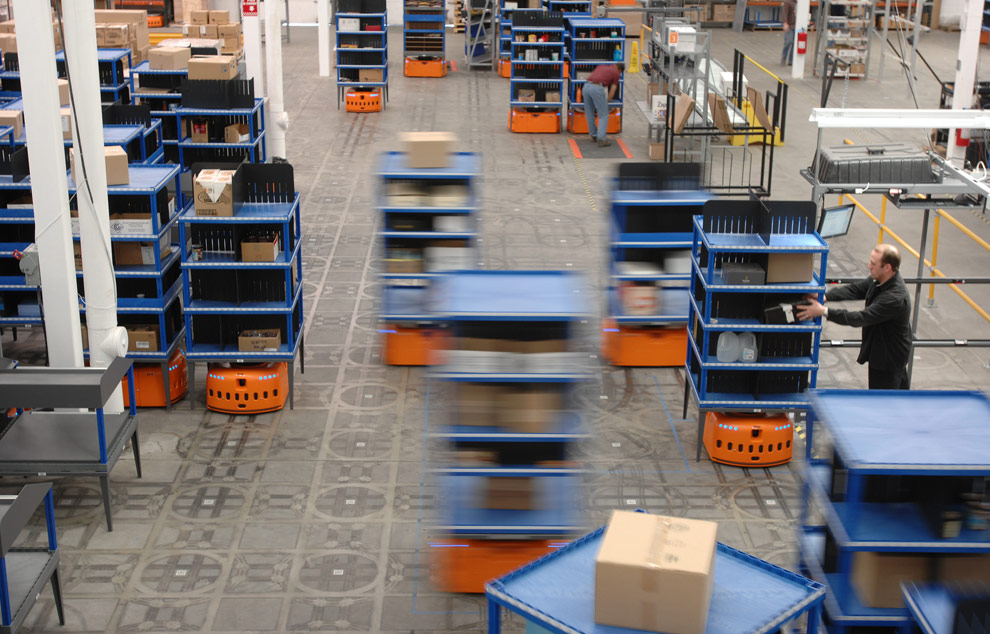
\includegraphics[width=\textwidth,height=0.65\textwidth]{pics/kiva}
\caption{The Kiva Warehouse System \textcolor{red}{ref}}
\label{fig:kiva}
\end{minipage}
\quad
\begin{minipage}[b]{0.5\linewidth}
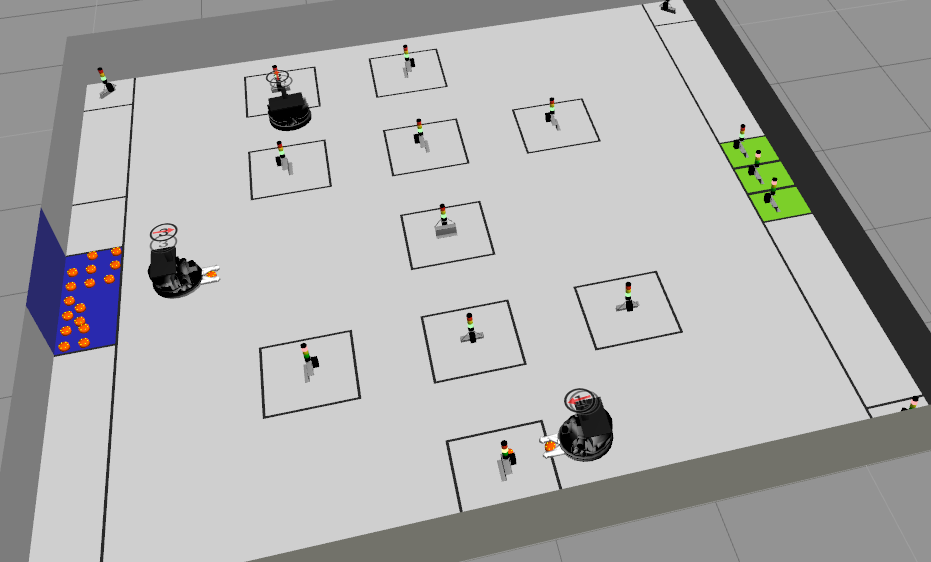
\includegraphics[width=\textwidth,height=0.65\textwidth]{pics/sim_working}
\caption{The LLSF simulated in Gazebo}
\label{fig:intro_sim}
\end{minipage}
\end{figure}
As the warehouse domain shows, multi-robot systems are efficient, flexible and can solve complex tasks. How important a multi-robot system can be was demonstrated by the acquisition of Kiva Systems for $\$775$ million by Amazon~\cite{kiva_amazon}. Beside warehousing, there are many more possible applications for multi-robot systems. In this thesis, we focus on a logistics domain in a factory environment. Here, robots manage the material and product flow between machines, what is more flexible and scalable than using a fixed assembly line. A testbed for multi-robot systems in this domain is the \textit{Logistic League sponsored by Festo (LLSF)}, which is part of the international robotics competition RoboCup and features the mobile robot platform \textit{Robotino}. We participate in this league with the \textit{Carologistics} team\footnote{\url{http://carologistics.org}}. Carologistics is a joint team consisting of the Knowledge-based Systems Group at RWTH Aachen University, the IMA/ZLW \& IFU Institute Cluster at RWTH Aachen University and the Department for Electrical Engineering and Information Technology, Robotics Group at FH Aachen. We operate our robots with the robot software framework \textit{Fawkes}. To achieve a multi-robot system with good performance, robust robot behavior and an efficient scheduling, we have a special need for a multi-robot simulation we developed in this thesis. This simulation should allow efficient evaluation and development of our high-level agent, which is responsable for decicion making and coordination with other robots. We decided to develop automated simulation runs to measure and compare the performance of the multi-robot system in different configurations. The simulation also has to be physically and visually realistic so that the robot software can run as in the real world. Instead of real sensor data, the robot software receives simulated sensor data and the actions the robot would take in reality are executed in the simulation. Furthermore, the simulation should be extendable for future changes of the robot or the environment.\\
Figure~\ref{fig:intro_sim} shows the Gazebo simulator, which we chose as a basis, and the simulation of the LLSF environment we developed during this thesis. With this simulation we are able to improve our multi-robot system because we can efficiently test and evaluate our changes. During a Hackathon, we provided our simulation in an adjusted version as a testing platform for a search and rescue scenario. With our simulation, about 40 inexperianced participants developed robot software, which sucessfully performed in reality altougth the testing possibilities on real robots were limited. 
\\
In chapter~\ref{cha:background}, we show the background of this thesis. This includes descriptions of the Robotino, the RoboCup and LLSF, Fawkes, Gazebo and other used tools. In chapter~\ref{cha:related_work}, we present related work about other simulations and agent strategies. Furthermore, we describe the current LLSF solution of the Carologistics team. The approach of this thesis is described in chapter~\ref{cha:approach}. In chapter~\ref{cha:implementation}, we present the implementation. This includes a description of the developed simulation modules and the improvements on our LLSF system. The evaluation results of the changes of the agent and the simulation itself are shown in chapter~\ref{cha:evaluation}. In chapter~\ref{cha:summery_and_future_work}, we suggest future work and conclude.



%% Multi-robot systems are combinations of multiple robots that work together on specific tasks. Currently, they are mostly used in assembly lines, where many robot-arms simultaneously do repetitive tasks on the same objects. More autonomous examples of multi-robot systems can be found in the warehouse domain. Here, many robots bring demanded goods from the storage and store new ones~\cite{Kiva}. The major advantages of multi-robot systems are high flexibility and the possibility to run different tasks in parallel. The amount of possible applications is large. Beside assembly and warehousing, they can also be used in rescue scenarios~\cite{mas_rescue}, soccer~\cite{mas_soccer}, planetary exploration~\cite{mas_space}, logistics and more.\\
%% Developing a robotic system is challenging. Robots have to detect objects, localize themselves, reason about their surrounding and manipulate it. Developing a multi-robot system is even harder because the robots have to do all these tasks in coordination with other robots. Furthermore, the systems have to be robust against the failure of single robots and should be as efficient as possible. Because of these challenges, testing is an essential part of the development process. It is necessary to identify mistakes in the source code and to evaluate how the system performs in a complex environment. Often, tests reveal problems the developer did not expected. However, testing can be difficult and time consuming for several reasons. The robot and the environment have to be available and set up. A component to be tested can depend on other components that are still being developed. Some tests require cautious execution because the robot could harm itself or the environment and full system tests have to run a longer time. Testing a multi-robot system is even harder. On the one hand the testing effort scales with the number of robots. On the other hand the system is more complex and therefore requires more test runs for evaluation.\\
%% In this thesis, we tackle these problems by developing a multi-robot simulation environment. This environment has to be physically and visually realistic. The robot software runs like in the real world and gets simulated sensor data instead of real sensor data. When the robot software uses actuators, the actions are executed in the simulation. This brings many advantages and can speed up the testing process. With a simulation environment, the majority of tests needs neither available robots nor the environment, the setup can be automated and unfinished components, that other components depend on, can be simulated as well. Furthermore, we want to evaluate the whole multi-robot system by measuring its performance in multiple runs. This enables us to easily compare different configurations and strategies in the simulation.\\
%% Such a simulation is useful in most robot developments. In this thesis we concentrate on the logistics domain and the mobile robot platform \textit{Robotino}. We participate in the \textit{Logistic League sponsored by Festo (LLSF)} with the \textit{Carologistics} team. The Carologistics is a joint team consisting of the Knowledge-based Systems Group at RWTH Aachen University, the IMA/ZLW \& IFU Institute Cluster at RWTH Aachen University and the Department for Electrical Engineering and Information Technology, Robotics Group at FH Aachen. LLSF is an industrially motivated competition within the RoboCup initiative. Three robots have to manage the material flow in a production area. The goal is to produce as many ordered products by feeding different machines in the production area with resources and intermediate products. To achieve a good performance, robust robot behavior and an efficient scheduling is necessary. Because of this, we have a special need for a multi-robot simulator, which can test the performance of single robots as well as the efficiency of the whole multi-robot system.\\
%% We use the \textit{Fawkes} robot software framework to control the robots and we choose \textit{Gazebo} as robot simulator. Important tasks of this thesis are the connection between Fawkes and Gazebo, the simulation of sensor data and the modeling of the LLSF environment and the actions of the robot in this environment. Because we want to use the multi-robot simulation to evaluate and improve our own LLSF system, we will also develop some concrete improvements and compare the performances of this system with different configurations. The majority of these improvements relate to the high level agent, which is responsible for the decisions of the robot and the coordination between the agents.
